% !TEX program = pdflatex
% Compile from docs/ so that "../outputs/..." paths resolve.
\documentclass[11pt]{article}

% ── Layout ────────────────────────────────────────────────────────────────────
\usepackage[margin=1in]{geometry}
\usepackage{microtype}
\usepackage{parskip}
% Let TeX stretch spacing as a last resort so unbreakable \code{} chips
% never spill past the right margin (clears overfull \hbox warnings).
\setlength{\emergencystretch}{3em}
\usepackage{float}           % [H] float specifier
\usepackage{tikz}
\usetikzlibrary{arrows.meta, positioning}

% ── Fonts ─────────────────────────────────────────────────────────────────────
\usepackage[T1]{fontenc}
\usepackage{lmodern}
\usepackage{newtxtext}
\usepackage[scaled=0.92]{inconsolata}

% ── Math / symbols ────────────────────────────────────────────────────────────
\usepackage{amsmath}
\usepackage{amssymb}

% ── Graphics, color, tables ───────────────────────────────────────────────────
\usepackage{graphicx}
\usepackage{xcolor}
\usepackage{booktabs}
\usepackage{array}
\usepackage{caption}
\usepackage{subcaption}

% ── Boxes for callouts ────────────────────────────────────────────────────────
\usepackage[most]{tcolorbox}

% ── Code listings ─────────────────────────────────────────────────────────────
\usepackage{listings}

% ── Hyperlinks ────────────────────────────────────────────────────────────────
\usepackage{hyperref}

% ── Color palette ─────────────────────────────────────────────────────────────
\definecolor{accent}{HTML}{2E5A88}        % deep blue
\definecolor{accentred}{HTML}{C44E52}     % warm red (diagram highlights)
\definecolor{softgray}{HTML}{F5F5F7}      % callout background
\definecolor{rule}{HTML}{B7C2D0}          % thin separator
\definecolor{codebg}{HTML}{F2F4F7}        % inline code background

% ── Section formatting ────────────────────────────────────────────────────────
\usepackage{titlesec}
\titleformat{\section}
  {\color{accent}\Large\bfseries\sffamily}
  {\thesection}{0.6em}{}
  [\vspace{-2pt}{\color{rule}\titlerule[0.6pt]}]
\titleformat{\subsection}
  {\color{accent}\large\bfseries\sffamily}
  {\thesubsection}{0.5em}{}
\titlespacing*{\section}{0pt}{1.4em}{0.6em}

% ── Caption styling ───────────────────────────────────────────────────────────
\captionsetup{font=small, labelfont={bf,color=accent}, skip=4pt}

% ── Hyperref styling ──────────────────────────────────────────────────────────
\hypersetup{colorlinks=true, linkcolor=accent, urlcolor=accent, citecolor=accent}

% ── Inline code ───────────────────────────────────────────────────────────────
\newcommand{\code}[1]{%
  \tcbox[on line, colback=codebg, colframe=codebg,
         boxrule=0pt, arc=2pt, left=2pt, right=2pt, top=0pt, bottom=0pt]
        {\ttfamily\small #1}}

% ── Listings style (shell commands) ───────────────────────────────────────────
\lstdefinestyle{shell}{
  basicstyle=\ttfamily\small,
  backgroundcolor=\color{codebg},
  frame=single, framerule=0.4pt, rulecolor=\color{rule},
  xleftmargin=6pt, xrightmargin=6pt, framexleftmargin=6pt,
  breaklines=true, columns=fullflexible, keepspaces=true,
  showstringspaces=false, aboveskip=6pt, belowskip=6pt,
  commentstyle=\color{accent}, morecomment=[l]{\#},
}

% ── Callout box ───────────────────────────────────────────────────────────────
\newtcolorbox{keybox}[1][]{
  enhanced, breakable,
  colback=softgray, colframe=accent,
  boxrule=0pt, leftrule=3pt,
  arc=2pt, left=10pt, right=10pt, top=6pt, bottom=6pt,
  fonttitle=\bfseries\sffamily\color{accent},
  #1
}

% ── Title block ───────────────────────────────────────────────────────────────
\title{\vspace{-2.0em}{\color{accent}\textsf{\bfseries A Neural Network for Authorship Stylometry}}}
\author{}
\date{}

\begin{document}
\maketitle
\vspace{-3.0em}

\noindent
\textit{Given a passage written by one of several known authors --- or by nobody
we know --- can we recover who wrote it from writing style alone? Where K-means
asked whether style \emph{clusters}, here we ask a supervised question: train a
neural network on labelled passages and let it learn the decision
boundaries between authors directly, including a boundary for ``none of the
above''.}

% =============================================================================
\section{Classifying Authors with an NN}
\label{sec:model}

\paragraph{The open-set task.}
A closed-set classifier assumes every passage was written by one of the known
authors. In the real world that assumption fails: a passage may come from an
\emph{unknown} author, and a closed-set model will confidently mislabel it as
whichever known author it resembles most. We therefore pose the problem as
\textbf{open-set} recognition from the outset: five known LessWrong authors plus
an explicit sixth class, \code{none\_of\_the\_5\_authors}, that the network must
learn to recognise.

\paragraph{Dataset and preprocessing.}
The five known authors are \code{Eliezer Yudkowsky}, \code{John Wentworth},
\code{Raemon}, \code{Scott Alexander}, and \code{Zvi}, with roughly 150 passages
each ($723$ passages in total). The ``none'' class is built from \textbf{15
other LessWrong authors} not among the five (\code{ricraz}, \code{benquo},
\code{abramdemski}, \code{sarahconstantin}, \code{holdenkarnofsky},
\code{gordon-seidoh-worley}, \code{screwtape}, \code{buck}, \code{turntrout},
\code{nunosempere}, \code{benito}, \code{petermccluskey}, \code{joe-carlsmith},
\code{adamshimi}, \code{tsvibt}), sampling 10 articles from each for
\textbf{150 ``none'' passages}. Merged, this gives \textbf{873 passages over 6
classes}.

From each passage we extract \textbf{107 stylometric features} spanning seven
groups: word/sentence-length statistics, vocabulary richness (type-token ratio,
hapax ratio, Yule~$K$, Simpson~$D$, Brun\'et~$W$, Honor\'e~$R$), function-word
frequencies, stylistic word-category rates, punctuation rates, coarse POS-tag
distributions, and character-level ratios. None of these depend on \emph{what} a
passage is about, only on \emph{how} it is written. Every feature is z-scored
with \code{sklearn}'s \code{StandardScaler} (mean 0, standard deviation 1)
before training. Crucially, the scaler is fit on the training split only and
then applied to the validation and test splits, so no test-set statistics leak into
training.

\paragraph{The classifier.}
A neural network (NN) maps a feature vector
$\mathbf{x}\in\mathbb{R}^{107}$ to a probability over the $K=6$ classes. Each
hidden layer applies an affine transform followed by the \textbf{ReLU}
nonlinearity,
\[
  \mathbf{h}^{(\ell)} = \mathrm{ReLU}\!\big(W^{(\ell)}\mathbf{h}^{(\ell-1)}
  + \mathbf{b}^{(\ell)}\big),
  \qquad \mathrm{ReLU}(z)=\max(0,z),
\]
with $\mathbf{h}^{(0)}=\mathbf{x}$. The final layer produces $K$ logits that a
\textbf{softmax} turns into class probabilities,
\[
  p_k(\mathbf{x}) = \frac{\exp(z_k)}{\sum_{j=1}^{K}\exp(z_j)},
\]
and training minimises the multi-class \textbf{cross-entropy} loss over the
training passages,
\[
  L = -\frac{1}{N}\sum_{i=1}^{N}\sum_{k=1}^{K}
      \mathbf{1}[y_i = k]\,\log p_k(\mathbf{x}_i).
\]
Weights are learned by backpropagation with the \textbf{Adam} optimiser
(\code{sklearn.neural\_network.MLPClassifier}, \code{solver="adam"}). All hidden
layers use 64 units; we vary only the \emph{number} of such layers.

\begin{figure}[H]
\centering
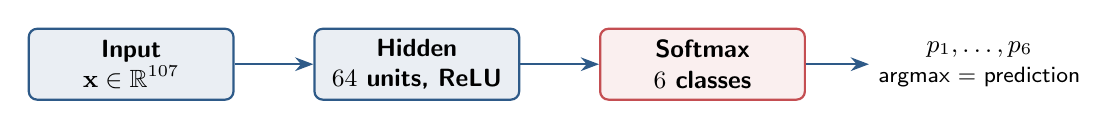
\begin{tikzpicture}[
  node distance=10mm,
  layer/.style={draw=accent, fill=accent!10, rounded corners=3pt,
    minimum width=2.6cm, minimum height=0.9cm, align=center,
    font=\small\sffamily\bfseries, thick},
  outlayer/.style={draw=accentred, fill=accentred!9, rounded corners=3pt,
    minimum width=2.6cm, minimum height=0.9cm, align=center,
    font=\small\sffamily\bfseries, thick},
  arr/.style={->, >=Stealth, accent, thick},
]
  \node[layer]    (in)  {Input\\$\mathbf{x}\in\mathbb{R}^{107}$};
  \node[layer, right=of in]  (h) {Hidden\\$64$ units, ReLU};
  \node[outlayer, right=of h] (out) {Softmax\\$6$ classes};
  \node[draw=none, right=8mm of out, font=\small\sffamily, align=center]
    (p) {$p_1,\dots,p_6$\\\footnotesize argmax = prediction};
  \draw[arr] (in)  -- (h);
  \draw[arr] (h)   -- (out);
  \draw[arr] (out) -- (p);
\end{tikzpicture}
\caption{The winning architecture: a single hidden layer of 64 ReLU units
feeding a $6$-way softmax (five known authors plus ``none''). Deeper variants
stack more 64-unit layers between input and output (Section~\ref{sec:depth}).}
\label{fig:arch}
\end{figure}

\paragraph{Training protocol.}
We split the 873 passages \textbf{60/20/20} (train / validation / test), stratified by
class, and use the validation split to choose a model before ever touching the test
split. Specifically we grid-search over three feature subsets (the top 30, top
50, and all 107 features) crossed with four network depths, training each
combination on the train split and scoring it on validation. The winner is then
\textbf{retrained on train$+$validation combined} and evaluated \emph{once} on
the held-out test set.

\paragraph{Which features?}
The top-30 and top-50 subsets are the most informative features as ranked by
\textbf{Random Forest permutation importance}: we fit a random forest
(\code{n\_estimators=500}, \code{max\_depth=5}) and measure, for each feature,
how much test accuracy drops when that feature's values are randomly shuffled.
Permutation importance is multivariate and redundancy-aware --- when several
stylometric features carry overlapping signal, it credits the one the forest
actually relies on --- so it is a sharper subset selector than scoring each
feature in isolation. As it turns out the distinction barely matters here: the
full 107-feature model wins on validation regardless, so the subsets serve only
to confirm that no small hand-picked group beats simply using everything.

\begin{figure}[H]
  \centering
  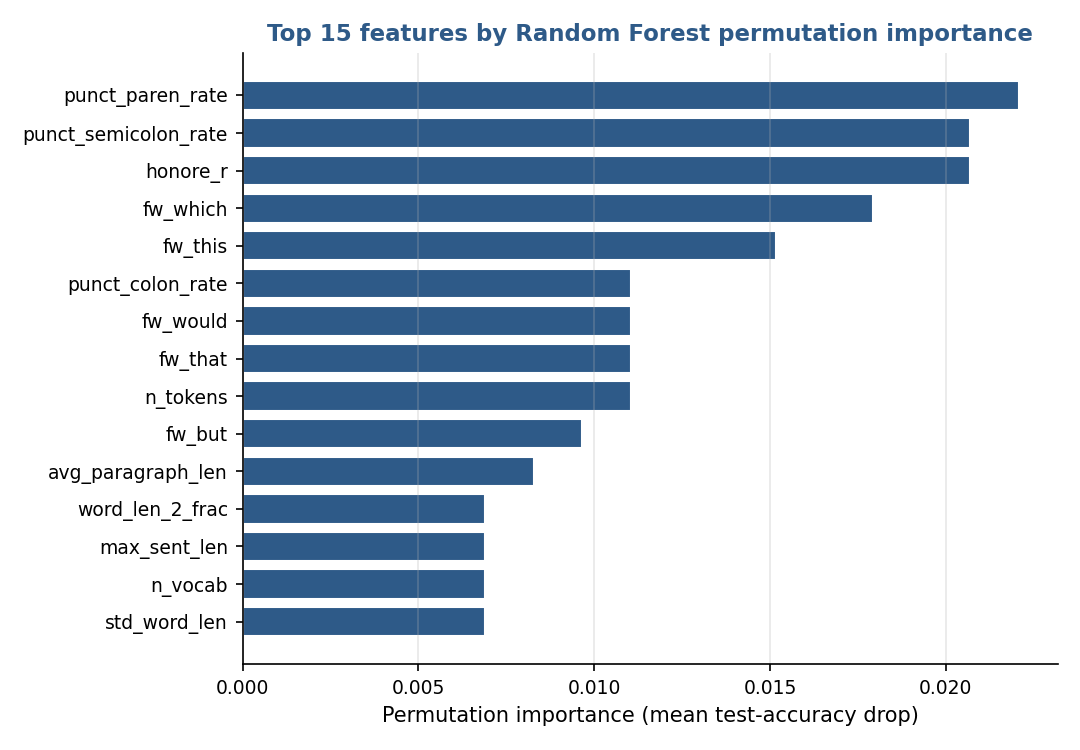
\includegraphics[width=0.72\linewidth]{../src/neural_network/outputs/rf_permutation_importance.png}
  \caption{The 15 most informative features by Random Forest permutation
  importance (mean drop in held-out accuracy when a feature is shuffled).
  Punctuation habits (parenthesis, semicolon, colon rates), a vocabulary-richness
  measure (Honor\'e's $R$), and a handful of function words (\code{which},
  \code{this}, \code{would}, \code{that}) dominate --- exactly the
  topic-independent, stylistic signals we want.}
  \label{fig:featimp}
\end{figure}

\begin{keybox}[title=Why early stopping?]
With only $\sim$520 training passages and thousands of weights, an NN can
memorise the training set. We pass \code{early\_stopping=True}: \code{sklearn}
holds out 10\% of the training data as an internal validation set and halts when
its score fails to improve for \code{n\_iter\_no\_change=15} consecutive epochs
(\code{batch\_size=32}, \code{max\_iter=500}). This curbs over-fitting and makes
the depth comparison fair --- every architecture is trained under the same
stopping rule.
\end{keybox}

\paragraph{Model selection on the validation set.}
Figure~\ref{fig:validation} shows validation accuracy for every feature-subset $\times$ depth
combination. The clear winner is \textbf{all 107 features with a single hidden
layer} (validation accuracy $0.943$). Two patterns already stand out: using all 107
features never hurts, and the deepest network (50 layers) collapses to chance
--- a phenomenon we return to in Section~\ref{sec:depth}.

\begin{figure}[H]
  \centering
  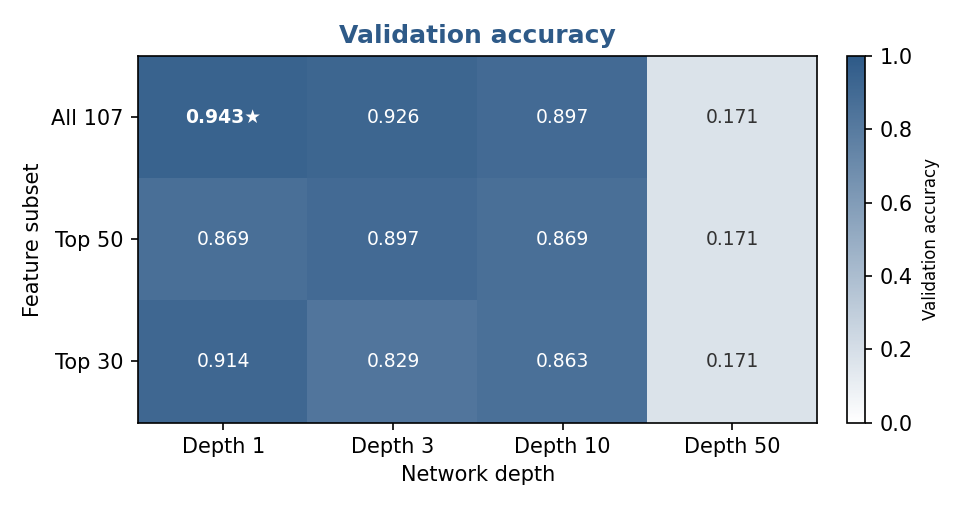
\includegraphics[width=0.78\linewidth]{../src/neural_network/outputs/validation_selection.png}
  \caption{Validation accuracy across feature subsets (rows) and network depths
  (columns). The starred cell --- all 107 features, depth 1 --- is the selected
  model. Depth 50 sits at $0.171$, barely above the six-class random baseline of
  $1/6\approx0.167$.}
  \label{fig:validation}
\end{figure}

\paragraph{Results.}
Retrained on train$+$validation (698 passages) and evaluated on the 175 test passages,
the selected model attains the scores in Table~\ref{tab:test}.

\begin{table}[H]
\centering
\caption{Test-set performance of the selected NN (all 107 features, depth 1).}
\label{tab:test}
\begin{tabular}{lc}
\toprule
\textbf{Metric} & \textbf{Value} \\
\midrule
Accuracy    & $0.949$ \\
Weighted F1 & $0.949$ \\
\bottomrule
\end{tabular}
\end{table}

The confusion matrix (Figure~\ref{fig:cm}) shows a strong diagonal. The striking
result is the \code{none\_of\_the\_5\_authors} class itself: \textbf{precision,
recall, and F1 are all $1.00$}. Not a single unknown-author passage is
misattributed to one of the five, and not a single known-author passage is
dumped into the ``none'' bin --- the 15 unknown authors, pooled together, occupy
a region of style-space cleanly separable from the five targets. Among the five
known authors the few errors concentrate on \code{Raemon} (recall $0.88$) and
\code{Scott Alexander} (recall $0.90$), whose passages are occasionally confused
with one another or with \code{Yudkowsky}; \code{Zvi} is recovered almost
perfectly.

\begin{figure}[H]
  \centering
  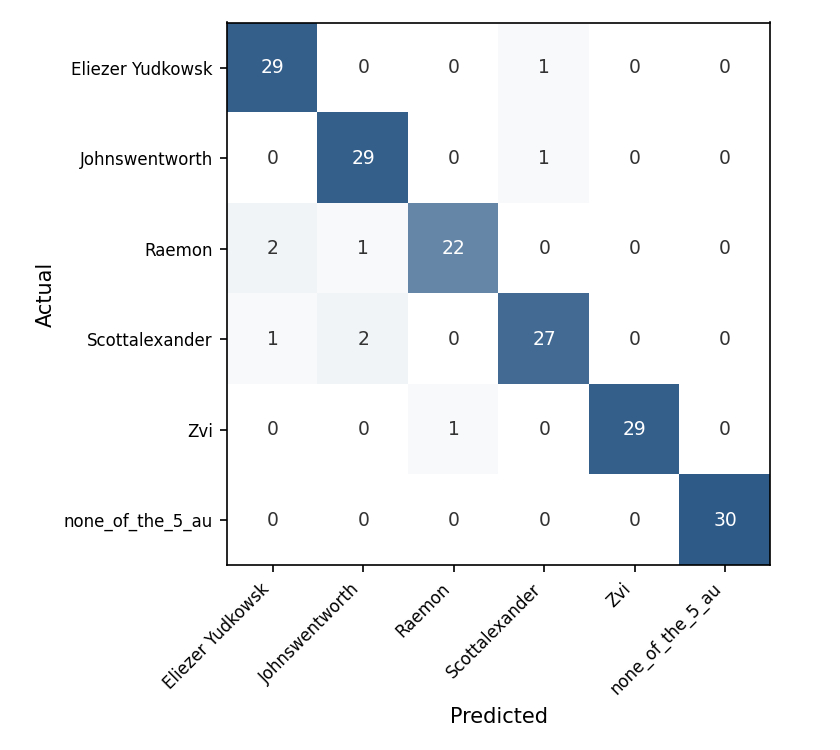
\includegraphics[width=0.56\linewidth]{../src/neural_network/outputs/confusion.png}
  \caption{Test-set confusion matrix (rows = actual, columns = predicted). The
  \code{none} row and column are perfectly isolated.}
  \label{fig:cm}
\end{figure}

\begin{keybox}[title=Direct training beats indirect thresholding]
Why add a class instead of simply flagging low-confidence predictions from a
closed-set five-author model as ``unknown''? We tried that indirect route,
thresholding the five-class softmax probabilities, and it failed completely:
unknown passages routinely produced \emph{high}-confidence predictions for one
of the five authors, so a confidence threshold caught essentially none of them.
Giving the network labelled ``none'' examples and letting it learn the boundary
directly is far more effective --- here, perfectly so. The contrast against 15
stylistically diverse ``other'' authors also appears to \emph{sharpen} the
boundaries among the five targets: the model learns not just what each target
author looks like, but what they do \emph{not} look like.
\end{keybox}

% =============================================================================
\section{How Deep Should the Network Be?}
\label{sec:depth}

A natural instinct is that deeper networks are more powerful, so they should
classify better. Our grid search says otherwise. Figure~\ref{fig:depth} plots
validation accuracy against depth for each feature subset.

\begin{figure}[H]
  \centering
  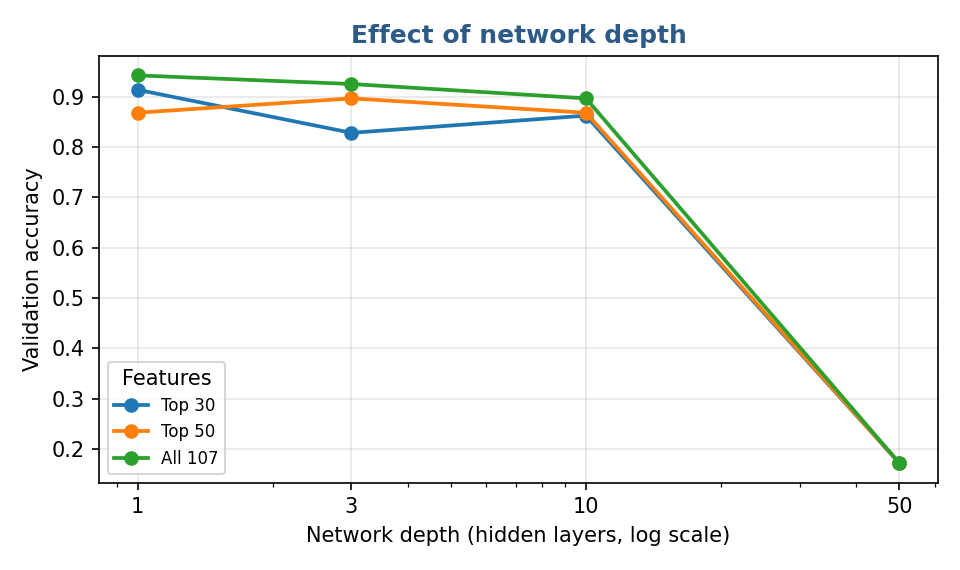
\includegraphics[width=0.7\linewidth]{../src/neural_network/outputs/depth_effect.png}
  \caption{Validation accuracy vs.\ network depth (number of 64-unit hidden layers, log
  scale). Performance is flat-to-slightly-declining from depth 1 to depth 10,
  then \textbf{collapses to chance at depth 50}.}
  \label{fig:depth}
\end{figure}

From depth 1 to depth 10 accuracy barely moves --- the extra layers buy nothing
because the decision boundaries between these classes are already well within
reach of a shallow network on 107 informative features. At depth 50 every
configuration collapses: validation accuracy falls to $0.171$, essentially the random
baseline of $1/6\approx0.167$. The network has stopped learning anything.

\begin{keybox}[title=Why the deep network fails]
This is not over-fitting --- an over-fit network would still score well above
chance on validation. It is an \emph{optimisation} failure. Stacking 50 plain
fully-connected ReLU layers with no residual connections or normalisation
produces vanishing gradients: the error signal is attenuated layer by layer
during backpropagation, so the early layers receive almost no useful gradient.
Combined with early stopping on a small dataset, training halts before the
network escapes its near-random initialisation. The lesson is concrete: for
tabular stylometric features, \textbf{a shallow NN is not just sufficient but
preferable}.
\end{keybox}

\paragraph{Are the gradients actually vanishing?}
The vanishing-gradient explanation is testable, so we test it. We re-implement
the same architecture in numpy --- Glorot-uniform initialisation with bound
$\sqrt{6/(\text{fan\_in}+\text{fan\_out})}$ (exactly what \code{sklearn} uses for
ReLU layers), ReLU hidden units, softmax output, cross-entropy loss --- and read
off the gradient of the loss with respect to every layer's weights from a single
forward/backward pass on the standardised features. Averaging over 50 random
initialisations, Figure~\ref{fig:grad} reports the root-mean-square (RMS) of the
weight gradients at each layer, at the moment training begins.

\begin{figure}[H]
  \centering
  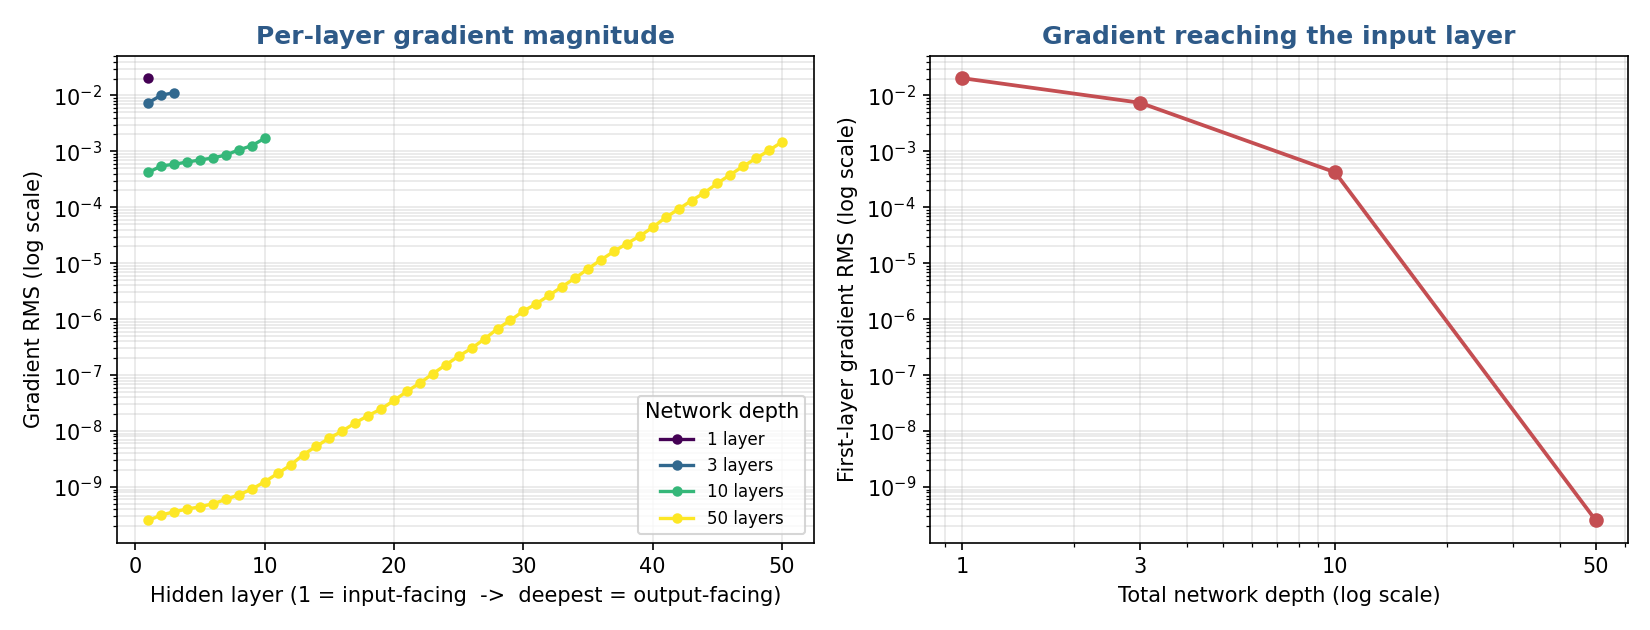
\includegraphics[width=0.95\linewidth]{../src/neural_network/outputs/gradient_health.png}
  \caption{Gradient health at initialisation. \textit{Left}: RMS weight gradient
  per layer, from the input-facing layer (1) to the output-facing layer, one
  curve per depth (log scale). \textit{Right}: the gradient reaching the
  input-facing first layer as a function of total depth. Both axes are
  logarithmic.}
  \label{fig:grad}
\end{figure}

The signature is unmistakable. In the shallow networks the gradient is roughly
uniform across layers --- at depth 1 the input layer already sees an RMS gradient
of $2.0\times10^{-2}$, only $3.5\times$ smaller than the output layer. As depth
grows the gradient decays geometrically on its way back to the input, so the
first layer is starved (Table~\ref{tab:grad}). By 50 layers the input-facing
layer receives an RMS gradient of $2.5\times10^{-10}$ --- eight orders of
magnitude weaker than in the shallow net, and $2\times10^{7}$ times weaker than
the output layer of the \emph{same} network.

\begin{table}[H]
\centering
\caption{RMS weight gradient at initialisation, averaged over 50 inits. The
first layer (input-facing) is the one that must learn feature combinations; its
gradient collapses with depth.}
\label{tab:grad}
\begin{tabular}{rccc}
\toprule
\textbf{Depth} & \textbf{First-layer grad} & \textbf{Output grad} & \textbf{Ratio (out\,/\,first)} \\
\midrule
1  & $2.0\times10^{-2}$  & $7.0\times10^{-2}$ & $3.5$ \\
3  & $7.4\times10^{-3}$  & $3.1\times10^{-2}$ & $4.2$ \\
10 & $4.2\times10^{-4}$  & $5.8\times10^{-3}$ & $13.7$ \\
50 & $2.5\times10^{-10}$ & $5.5\times10^{-3}$ & $2.2\times10^{7}$ \\
\bottomrule
\end{tabular}
\end{table}

A weight that sees a gradient of $10^{-10}$ cannot move: with early stopping
monitoring a validation score that never improves, training halts within a few
epochs and the deep network never leaves its random initialisation --- which is
exactly the chance-level accuracy we saw at depth 50. This confirms the collapse
is an \emph{optimisation} pathology, not a capacity or over-fitting one. The
standard fixes (residual connections, batch/layer normalisation, He
initialisation) all exist precisely to keep this gradient alive; none are
warranted here, because the shallow network already solves the task.

% =============================================================================
\section{Conclusion}

A deliberately simple model --- a single hidden layer of 64 ReLU units on 107
z-scored stylometric features --- attributes LessWrong passages to one of five
authors or to an open-set ``none of the above'' class with $95\%$ accuracy,
recognising the unknown-author class \emph{perfectly}. Depth does not help and,
past a point, destroys the model outright. The supervised picture is sharper
than the unsupervised one: where K-means recovered ten-author structure at
ARI~$\approx 0.55$, a labelled NN separates a handful of authors almost
cleanly, confirming that the stylistic signal is strong and largely
linearly-accessible once the right features are in hand.

% =============================================================================
\section{Setup and Reproducibility}
\label{sec:setup}

All experiments run on CPU in well under a minute each. The module lives in
\code{src/neural\_network/}, organised into \code{data/} (the feature CSV and
the \code{cleaned\_5} / \code{cleaned\_35} article sets), \code{scripts/} (all
Python), and \code{outputs/} (every figure plus \code{results.md}). The report
figures are produced by \code{make\_report\_figures.py} and
\code{gradient\_diagnostics.py}.

\paragraph{Dependencies.}
Python~$\geq 3.10$ with a handful of scientific packages:
\begin{itemize}\setlength\itemsep{1pt}
  \item \code{numpy}, \code{pandas} --- data handling
  \item \code{scikit-learn} --- \code{MLPClassifier}, splitting, scaling, metrics
  \item \code{matplotlib} --- all figures
  \item \code{nltk} --- tokenisation / POS-tagging when building the ``none''
        class from raw articles (a regex fallback is used if NLTK data is
        unavailable)
\end{itemize}

\paragraph{Install.}
From the project root, ideally inside a virtual environment:
\begin{lstlisting}[style=shell]
# from the project root; a virtual environment is recommended
python -m venv .venv
.venv\Scripts\activate          # Windows  (use: source .venv/bin/activate on macOS/Linux)
pip install numpy pandas scikit-learn matplotlib nltk
\end{lstlisting}

\paragraph{Run the model.}
The script builds the ``none'' class, merges, trains the full feature-subset
$\times$ depth grid, selects on the validation split, retrains the winner, and writes
\code{results.md} into \code{outputs/}.
\begin{lstlisting}[style=shell]
cd src/neural_network/scripts
python neural_network_code.py     # -> ../outputs/results.md
\end{lstlisting}

\paragraph{Regenerate the report figures.}
This reproduces the validation-selection heatmap, the depth-effect plot, and the
confusion matrix into \code{src/neural\_network/outputs/}. The gradient-health
diagnostic (Figure~\ref{fig:grad}, Table~\ref{tab:grad}) is a separate script.
\begin{lstlisting}[style=shell]
cd src/neural_network/scripts
python make_report_figures.py      # validation selection, depth, confusion
python gradient_diagnostics.py     # per-layer gradient health -> gradient_health.png
\end{lstlisting}

\paragraph{Compile this report.}
Run \code{pdflatex} from the \code{docs/} folder (twice, so cross-references and
the table of figures resolve):
\begin{lstlisting}[style=shell]
cd docs
pdflatex neural_network_report.tex   # run twice to resolve cross-references
\end{lstlisting}

\end{document}
